El dise'no de la aplicaci'on es extremadamente modular. Hay dos m'odulos claramente diferenciados: por un lado tenemos la aplicaci'on residente en el PDA y por otro la aplicaci'on que ejerce de servidor, alojada en el ordenador central del hospital, donde tambi'en se aloja la base de datos.\bigskip \\ En la figura \ref{fig:dclasesPDA}, mostramos el diagrama de clases del MIDlet que implementa la aplicaci'on del PDA. Consta de un 'unico MIDlet, PdaMIDlet, y tiene varias clases auxiliares, PantallaInicio, MenuPrincipal, MenuImprimir y ConsultaExpediente,  con las que se implementan las distintas pantallas que se muestran en la aplicaci'on. Desde PdaMIDlet se llama a la primera pantalla (PantallaInicio) y ellas se comunican entre s'i a trav'es de m'etodos de PdaMIDlet.

\begin{figure*}[h!]
	\begin{center}
        		\framebox{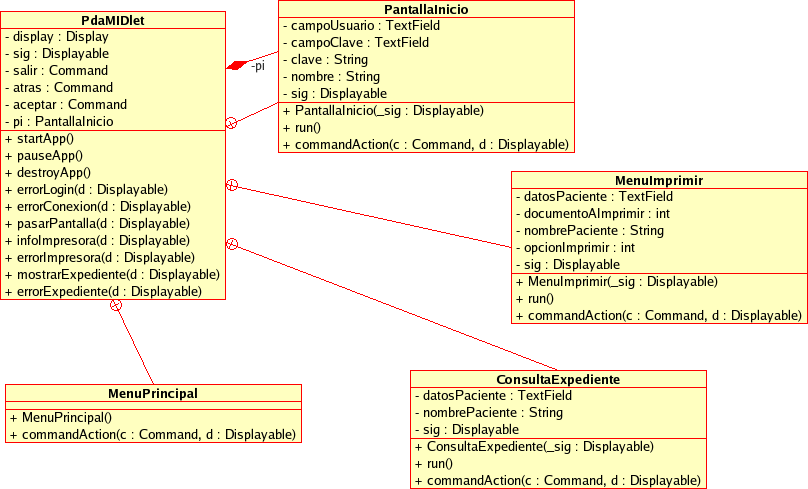
\includegraphics[scale=0.55]{dclasesPDA.png}}
     	\end{center}
    	\caption{Diagrama de clases de la aplicaci'on residente en el PDA}
	\label{fig:dclasesPDA}
\end{figure*}
En el servidor tenemos varias partes:
\begin{itemize}
	\item Base de datos
	\item Localizador de personal: triangulador
	\item Localizador de dispositivos: mapa
\end{itemize}
Tenemos clases que aportan tipos de datos como: 
\begin{itemize}
	\item Antena: modela los puntos de acceso
	\item Punto: modela las posiciones del personal en el hospital
	\item Nodo: modela los nodos del grafo de salas
\end{itemize}
Adem'as est'a la clase JavaServer que contiene la parte de la aplicaci'on que recibe las llamadas de la PDA.
En las figuras \ref{fig:dclasesServidor1} y \ref{fig:dclasesServidor2} se muestra el diagrama de clases de la aplicaci'on residente en el servidor.

\begin{figure*}[h!]
	\begin{center}
		\framebox{\includegraphics[scale=0.3]{dclasesServidor1.png}}
     	\end{center}
    	\caption{Diagrama de clases de la aplicaci'on residente en el Servidor: la base de datos}
	\label{fig:dclasesServidor1}
\end{figure*}

\pagebreak 

\begin{figure*}[h!]
	\begin{center}
		\framebox{\includegraphics[scale=0.3]{dclasesServidor2.png} }
     	\end{center}
    	\caption{Diagrama de clases de la aplicaci'on residente en el Servidor (sin base de datos)}
	\label{fig:dclasesServidor2}
\end{figure*}